\documentclass[a4paper,11pt]{refart}

\usepackage[utf8]{inputenc}
\usepackage[T1]{fontenc} % LY1 also works

%% Font settings suggested by fbb documentation.
\usepackage{textcomp} % to get the right copyright, etc.
\usepackage[lining,tabular]{fbb} % so math uses tabular lining figures
\usepackage[scaled=.95,type1]{cabin} % sans serif in style of Gill Sans
\usepackage[varqu,varl]{zi4}% inconsolata typewriter
\useosf % change normal text to use proportional oldstyle figures
%\usetosf would provide tabular oldstyle figures in text

\usepackage{microtype}

\usepackage{graphicx}
\usepackage{enumitem}
\setlist{leftmargin=*}
\usepackage{listings}
\lstset{basicstyle=\ttfamily,frame=single,xleftmargin=3em,xrightmargin=3em}
\usepackage[os=win]{menukeys}
\renewmenumacro{\keys}[+]{shadowedroundedkeys}
\usepackage{framed}
\usepackage{etoolbox}
\AtBeginEnvironment{leftbar}{\sffamily\small}
\usepackage{nameref}
\usepackage{siunitx}
\usepackage{float}
\usetikzlibrary{chains,arrows,shapes,positioning}
%\usepackage{hyperref}
\usepackage[hidelinks]{hyperref}

\newcommand\AutoCalc{\textsf{AutoratingCalculator}}
\renewcommand\abstractname{Introduction}

\title{Long Term Statistics toolbox for ArcGIS - User Guide}
%\author{Lim Lian Tze (\url{liantze@gmail.com})\\\url{http://liantze.penguinattack.org}}
\date{\url{https://enielsen93.github.io/enielsen93/LTS-Toolbox.html}}
\begin{document}
	\maketitle
	
	\begin{abstract}
	Long Term Statistics toolbox is a tool to develop DHI MIKE Urban LTS-files (Long Term Statistics) through ArcGIS.
	
	The tool is compatible with all versions of ArcGIS and can use both .dfs0-files from MIKE Urban or .km2-files from the rain gauge system of Spildevandskomitéen. It can write LTS-files for use in long term simulations through Mike Urban. 
	\end{abstract}
	
	\tableofcontents
	\clearpage
	
%	\section*{Quick Guide to Workflow}
%	
%	%\begin{enumerate}
%	%\item 
%	%\end{enumerate}
%	
%	\begin{tikzpicture}
%	\tikzset{every node/.style={on chain,draw,thick,rounded corners,
%			minimum height=3em, text width=10em, align=center}}
%	\begin{scope}[start chain=going below]
%	\node (prepare-group) {Prepare group list (\texttt{.csv})};
%	\node (import-group) {Import group list for new score file (\texttt{.xml})};
%	\node (enter-rating) {Enter peer ratings given by each student};
%	\node (compute-score) {Compute autorated weights and scores};
%	\node (export-csv) {Export data for Excel (\texttt{.csv})};
%	\end{scope}
%	\node[right=of enter-rating] (open-score) {Open previously saved score file (\texttt{.xml})};
%	
%	\path[draw,line width=0.4ex, ->,>= angle 60]
%	(prepare-group) edge (import-group) 
%	(import-group) edge (enter-rating)
%	(open-score) edge (enter-rating)
%	(enter-rating) edge (compute-score) 
%	(compute-score) edge (export-csv);
%	\end{tikzpicture}
	
	
	\section{Field descriptions}
	The user interface of the tool `Create LTS-file' is seen on figure \ref{fig:Fields}. The different fields are described in the following.
	\begin{figure}[hbt!]\centering
		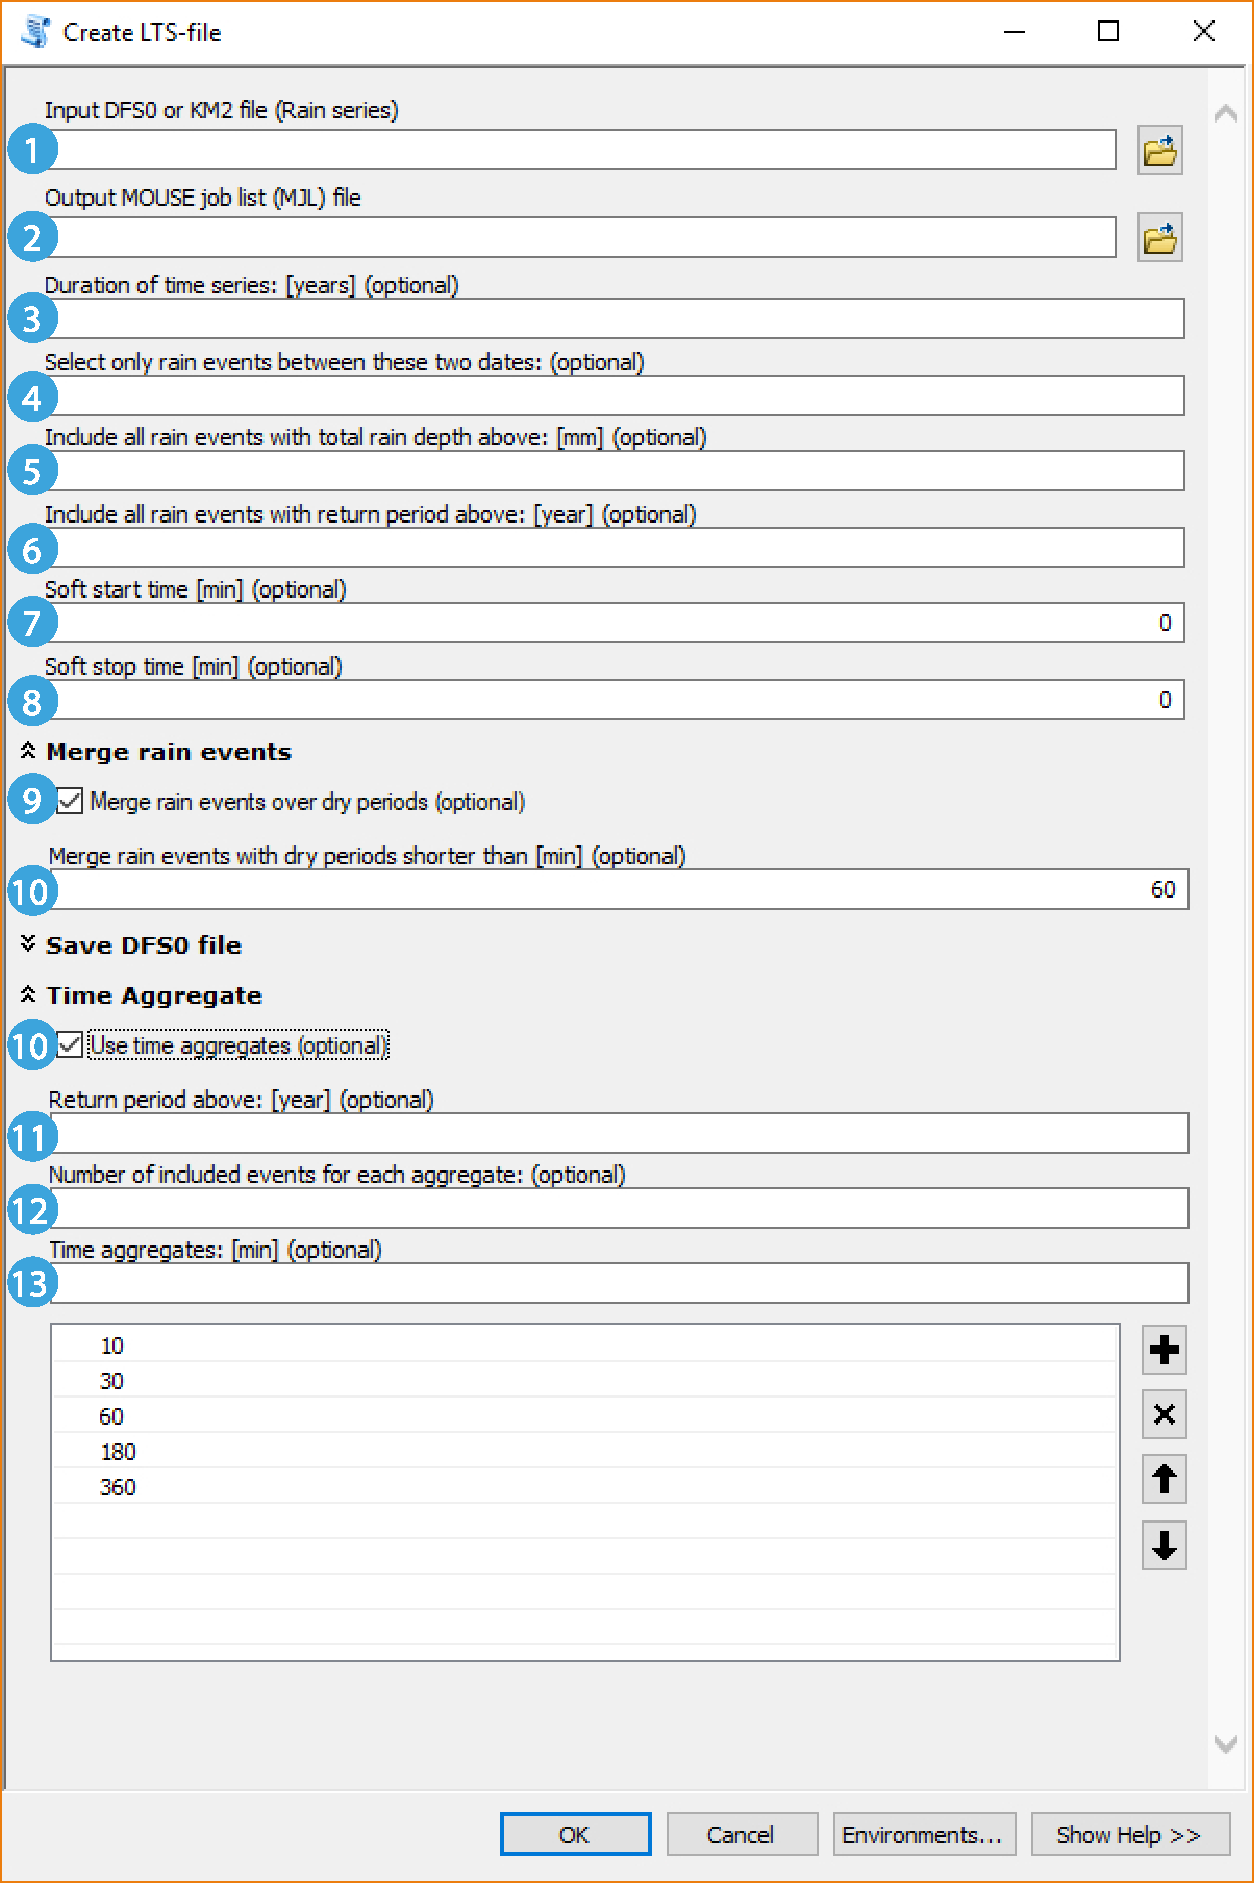
\includegraphics[scale=0.45]{Fields.pdf}
		\caption{The user interface}\label{fig:Fields}
	\end{figure}
	\subsection{Input DFS0 or KM2 file (Rain series)}
	\label{field1}
	Select the DFS0 or KM2 file that you wish to generate an LTS file for. DFS0 files can be generated through Mike Urban, and KM2 files are available from \url{http://svk.dmi.dk} (requires SVK license to access).
	
	\subsection{Output MOUSE Job list (MJL) file}
	Select the path and filename for the MOUSE job list (LTS-file) that you wish to generate. \textit{Overwriting existing MJL files is not permitted.}
	
	\subsection{Duration of time series}
	\label{field3}
	The duration of the time series is calculated for an input DFS0 or KM2 file immediately after selecting one in field `\nameref{field1}'. If the calculated time period is incorrect, replace the calculated number with your own. \textit{Calculation of duration of time series does not account for gaps in the time series, e.g. from rain gauge failure. If the actual duration of time series is known, replace the calculated value with this in [years]}
	
	The duration of the time series is used for calculating the return period for each rain event, which is used in field `\nameref{field6}' and `\nameref{fiield11}'.
	
	\subsection{Select only rain events between these two dates}
	Insert the two dates that you wish to include rain events from. Example: If you wish to include only rain events in the years 2008 and 2009, write `2008 - 2010' or `01/01/2008 - 01/01/2010'.
	
	\textit{Default value is the start and end date of the input time series.} 
	
	\subsection{Include all rain events with total rain depth above}
			\label{field5}
	Includes all rain events with total rain depth above a certain rain depth. 	Example: If input value is 2, all rain events with a total rain depth above \SI{2}{mm} will be included in the LTS-file. If the field is left empty, no rain events will be included from this method. 
	
	\textit{Can not be used simultaneously with field '\nameref{field6}'.}
	
	\subsection{Include all rain events with return period above}
		\label{field6}
	Includes all rain events with with a return period above a certain extent. E.g. if input value is 5, all rain events with a return period above \SI{5}{years} are included in the LTS-file. Return period is calculated from the total rain depth of an event. 
	
	The ranking of each rain event is according to the total rain depth of the event. Thus the event with the greatest rain depth is assigned a return period of the duration of the time series, seen in field `\nameref{field3}'. The event with the 2nd greatest rain depth is assigned a return period corresponding to half the duration of the time series etc. 
	
	The return period of a rain event is calculated from the following formula:
	\begin{equation}
		RP = \frac{dur_{\text{time series}}}{rank}
		\end{equation}
	Where:
	
	\begin{tabular}{r|l}
		$RP$ & Return period of an event\\
		$dur_{\text{time series}}$ & Duration of time series\\
		$rank$ & Rank of rain event according to rain depth (greatest is 1)
		\end{tabular}
	
	\textit{Can not be used simultaneously with field '\nameref{field5}'.}
	\subsection{Soft start time}
	Soft start time of LTS simulation. If input value is 60, the LTS simulation will include 60 minutes prior to the beginning of a rain event, including whatever rain may fall in that period. 
	
	\textit{This period is not included in the evaluation of the total rain depth or the return period for an event.}
	
	\subsection{Soft stop time}
	Soft stop time of LTS simulation. If input value is 60, the LTS simulation will include 60 minutes after the end of a rain event, including whatever rain may fall in that period. 
	
	\textit{This period is not included in the evaluation of the total rain depth or the return period for an event.}
	
	\subsection{Merge rain events over dry periods}
	Check this field if you wish to merge rain events that are separated by a dry period. Maximum allowed duration of the dry period if they're to be merged is selected in field `\nameref{field10}'. 
	
	\subsection{Merge rain events over dry periods}
	\label{field10}
	Merge rain events if they're separated by a dry period below the input value. Example: If two rain events are separated by a dry period of 120 minutes, and the input value is 160, these two rain events will be merged - this means that the total rain depth of the event and the time aggregates will be calculated across both rain events. 
	
	An illustration of this feature is shown in \ref{fig:RainEventPatterns2}. The rain depth, return period, and time aggregates are calculated across both rain events if the input value is above 120 min. If not, then the two rain events are considered separate. 
	
	\begin{figure}[H]\centering
		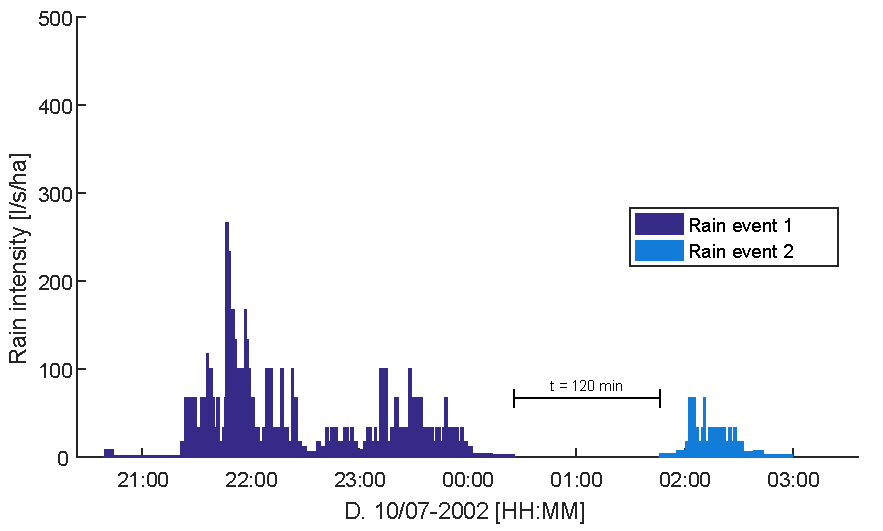
\includegraphics[scale=0.7]{RainEventPatterns2.pdf}
		\caption{Illustration of the effect of merging rain events.}\label{fig:RainEventPatterns2}
	\end{figure}
	
	\subsection*{Save DFS0 file}
	\textit{Feature no longer supported. Do not change anything here. }
	\subsection{Use time aggregates}
	Check this field if you wish to select and include rain events according to the accumulated rain depth over a defined period. 
	\subsection{Return period above}
	\label{fiield11}
	Includes all rain events whose return period according to rain depth over each input time aggregate period is above input value. 
	See field \nameref{field6}, except total rain depth is replaced with rain depth over time aggregate period.

For a time series with a total duration of 10 years, with 6 selected time aggregate periods, if the input return time is 5 years, then the total amount of included rain events is $2\cdot 6 = 12$. Because some rain events will most likely contain multiple time aggregates with a high return period, the actual amount of included events will be significantly less than 12.
		\subsection{Number of included events for each aggregate}
		Includes a specific amount of events that rank highest in rain depth over time aggregate period. 
		
		If input value is 12, with 6 selected time aggregate periods, then the total amount of included events is $12\cdot 6 = 72$. Because some rain events will most likely contain multiple time aggregates with a high return period, the actual amount of included events will be significantly less than 72.
		
		\subsection{Time aggregates}
		List of time aggregates for which events will be included for. Write a value into the field box and click the plus icon to add it. Select a value from the list and click the cross to delete this period. 
		
		An illustration of the time aggregate period is shown in figure \ref{fig:RainEventPatterns}. Two rain events are shown, and for this illustration the input values for time aggregates are 30 min, 60 min, 1480 min, 360 min, and 1440 min. Two events are separated by a period of 2 hours, but because the duration of the dry period is less than the greatest value for time aggregate period, the two events are merged. 
		\begin{figure}[H]\centering
			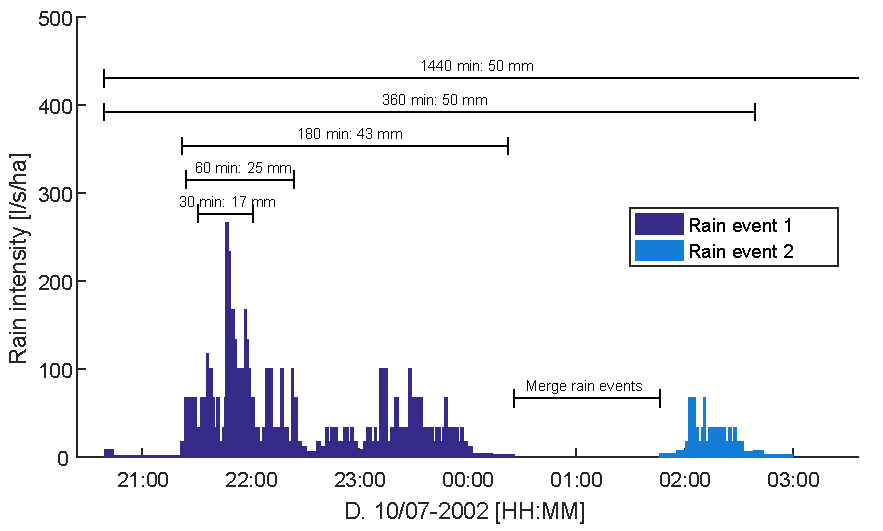
\includegraphics[scale=0.7]{RainEventPatterns.pdf}
			\caption{Illustration of the effect of merging rain events.}\label{fig:RainEventPatterns}
		\end{figure}
	\newpage
	\newpage
	
	
	\begin{enumerate}
		\item In Notepad, compile the list of group members in your class, using the following format:
		
		\begin{lstlisting}
		10032,Mary Tan
		10143,Prabakar Murugan
		10033,Tan Beng Huat
		10165,Calvin Ong
		
		10052,Mooi Siok Lan
		10114,Bong Chin Keat
		10432,Joseph Calvin
		10281,Suresh Kappan
		\end{lstlisting}
		
		\begin{itemize}[noitemsep]
			\item Record the \emph{ID} and \emph{name} of a student on each line.
			\item Use a comma (\texttt{,}) to separate the ID and name on each line.
			\item Leave an \emph{empty line} between groups.
		\end{itemize}
		
		\item Save the group list file using \texttt{.txt} or \texttt{.csv} extension, e.g.\\\texttt{DIT1234-Apr2013-groups.txt}.
		
		\medskip
		
		\begin{leftbar}
			You may also prepare the group list in Excel. List the IDs in column A and the IDs in column B. Save the file as a Comma separated values file (CSV). In the Export Filter Settings, set text delimiter to blank, and field separator to comma (\texttt{,}).
		\end{leftbar}
		
	\end{enumerate}
	
	\section{Importing a Group List for a New Assignment Score File}
	
	\begin{enumerate}
		\item Launch the \AutoCalc\ tool by double-clicking on its icon in Windows Explorer.
		\item From the menu bar, select \menu{File>Import...} or press \keys{Ctrl+I}.
		\item Select a \emph{group list file} (\texttt{*.txt, *.csv}) to import from, e.g.\\\texttt{DIT1234-Apr2013-groups.txt}.
		\item \AutoCalc\ will then ask you for a \emph{new} file name to save the new score list as (\texttt{*.xml}), e.g.~\texttt{DIT1234-Apr2013-Assgn1.xml}.
		
		
		\medskip
		
		\begin{leftbar}
			Make sure the \texttt{.xml} score filename selected does not already exist. Otherwise the existing score file \textbf{may be overwritten without warning}!
		\end{leftbar}
		
		\medskip
		
		\item \AutoCalc\ imports the group lists and displays the student IDs and names in the main panel (Figure~\ref{fig:grouplist}).
		
		\begin{figure}[hbt!]\centering
%			\includegraphics[width=\textwidth]{grouplist}
			\caption{Imported group list}\label{fig:grouplist}
		\end{figure}
	\end{enumerate}
	
	\section{Computing Autorated Scores from Group Scores and Peer Ratings}
	
	\subsection{Setting Options}
	
	Two options may be set at the top of the main \AutoCalc{} window.
	
	\begin{itemize}
		\item You may set the minimum and maximum autorating weight caps. Defaults are set at 0.8 and 1.02.
		
		\item You may choose whether to include self-evaluated peer ratings. The default is to include self ratings.
		
		\item If you change the settings, make sure to save them from the menu \menu{File>Save} or pressing \keys{Ctrl+S}.
	\end{itemize}
	
	\subsection{Selecting Students from List}
	
	Double-click on the name of a student in the list to display the peer review score entry window.
	
	\subsection{Searching Students by ID}
	
	You can also load the peer ratings entry window of a student by keying in the ID number in the search box, and then click on the \keys{Search} button.
	
	\subsection{Entering Scores and Ratings}
	
	\begin{enumerate}
		\begin{figure}[hbt!]
%			\includegraphics[width=\textwidth]{scorewindow}
			\caption{Peer Ratings Window}
		\end{figure}
		
		\item In the peer ratings window for each student, enter the peer ratings given by the student to his/her teammates, including him/herself.
		\item Enter also the overall score awarded to the group at the top of the window. (You only need to enter the group score once for each group.)
		\item Click the  \keys{Commit Ratings} button to save the ratings.
		\item Close the current peer rating window. Continue entering scores for other students.
		\item You may click on the \keys{Peer Ratings Received by \ldots} tab to see ratings received by a student.
		
		\begin{figure}[hbt!]
%			\includegraphics[width=\textwidth]{ratingsreceived}
			\caption{Peer Ratings Received}
		\end{figure}
		
	\end{enumerate}
	
	\subsection{Computing Autorated Scores}
	\begin{enumerate}
		\item When peer ratings of all students in a group has been entered and committed, click on the \keys{Compute Weights and Scores} button. The computed weights and scores will be saved to file immediately.
		\item Click on the \keys{Group Overview} tab to see autorated weights and scores for each student in the group.
		
		\begin{figure}[hbt!]
%			\includegraphics[width=\textwidth]{groupoverview}
			\caption{Autorated Weights and Scores of Group Members}
		\end{figure}
		
	\end{enumerate}
	
	\section{Opening Existing Assignment Score File}
	You may open an existing assignment score file (\texttt{*.xml}) to inspect scores, as well as to change settings and recalculate scores.
	\begin{enumerate}
		\item To open an existing score file, access the menu item \menu{File>Open\ldots} or press \keys{Ctrl+O}.
		\item Locate and select the \texttt{*.xml} file to open.
	\end{enumerate}
	
	\section{Exporting Data for Excel}
	The autorated scores can be exported for further processing in Excel.
	\begin{enumerate}
		\item Select \menu{File>Export\ldots} from the menu, or \keys{Ctrl+E}.
%		\item Select a file name to save the exported data in. The file will be saved with a \texttt{.csv} extension. \includegraphics[height=1em]{csv}
		\item In Windows Explorer, locate the \texttt{.csv} file and double-click on it to open it in Excel.
		\item If warning messages are displayed, keep on clicking \keys{OK} or \keys{Yes} to ignore them.
		\item When the data is displayed, you may save the file as an \texttt{.xlsx} or \texttt{.xsl} Excel file, and continue processing it.
		
		\begin{figure}[hbt!]
%			\includegraphics[width=\textwidth]{excel}
			\caption{Exported data in Excel}
		\end{figure}
		
	\end{enumerate}
	
	\bibliographystyle{plain}
	\bibliography{refs}
\end{document}